\section{Participatory Survey Results}
\label{sec:qual_results}

\begin{table*}[!t]
\centering
\caption{Past use (select all that apply) and choice of each data deletion method, in the less sensitive scenario (LS), the more sensitive scenario (MS), and both combined (Pooled). Choice is among the methods a participant had used, and choices of Other are left out.}
\label{tab:method-use}
\small
\begin{tabular}{@{}lrrrr@{}}
\toprule
 & Used & \multicolumn{3}{c}{Chosen} \\
\cmidrule(lr){3-5}
Method & ($n=177$) & LS & MS & Pooled ($n=352$) \\
\midrule
Sending a deletion-request prompt & 55 (31.1\%) & 25 & 14 & 39 (11.1\%) \\
Deleting a single conversation & 136 (76.8\%) & 84 & 80 & 164 (46.6\%) \\
Clearing all conversation history & 94 (53.1\%) & 33 & 40 & 73 (20.7\%) \\
Deleting a specific saved memory & 57 (32.2\%) & 19 & 22 & 41 (11.6\%) \\
Clearing all saved memories & 45 (25.4\%) & 7 & 8 & 15 (4.3\%) \\
Using a privacy dashboard & 17 (9.6\%) & 6 & 9 & 15 (4.3\%) \\
Deleting the account & 18 (10.2\%) & 2 & 3 & 5 (1.4\%) \\
Filing a request & 5 (2.8\%) & 0 & 0 & 0 (0.0\%) \\
\bottomrule
\end{tabular}
\end{table*}

Participants delete data at the conversation level, and more sensitive data raise their willingness to delete but not their choice of method. They expect the deletion to be permanent and often cannot check that it worked. This section reports these findings from the 177 participants; where we combine both scenarios (Pooled), percentages are of the 354 responses, or of 352 where choices of Other are left out.

\subsection{User Experience about Data Deletion}


Participants relied on conversation-level deletion and found the options on their own. Deleting a single conversation was the most used and the most chosen data deletion method, while methods that act on saved memories had been used by about a third of participants or fewer, and the account, the privacy dashboard, and filing a request by about one in ten or fewer (Table~\ref{tab:method-use}). Most participants found the options by browsing the settings or by guessing, and the agent told only 6 of 177. So most participants learned what they can delete without the agent's help.

Sensitivity changed how much participants wanted to delete, not how. In both LS and MS, most participants would probably or definitely delete the data (125 of 177 and 150 of 177), and willingness rose with sensitivity (mean 3.98 to 4.37 on the five-point scale; Wilcoxon signed-rank test, $p<.001$, $r=.55$). We found no change in which data deletion method participants chose between the scenarios (Stuart-Maxwell test, $p=.39$, 176 participants). So we found no sign that participants who wanted to delete more chose a different method.

Participants would prefer to ask the agent to forget, but seldom chose to. Asking the agent to forget was the second most often named ideal data deletion method, after deleting a single conversation (named by 47\% to 50\% of participants across LS and MS), yet only 8\% to 14\% of participants chose it. So the method participants name as ideal is not the one they use.

\subsection{User Expectation about Data Deletion}

Participants expected deletion to be permanent, and we found no difference in this between data deletion methods. Across Pooled responses, 59.0\% expected permanent deletion from the database and backups, and 54.2\% expected the fact never to come up in future conversations (Figure~\ref{fig:expectation}). The four most chosen methods differed in effort ($p_{\mathrm{Holm}}=.0001$) but not in protection ($p_{\mathrm{Holm}}=.29$; Figure~\ref{fig:scales}). Participants chose their own method and the groups are small, so these are associations. So participants distinguish the methods by effort, not by what they expect them to do.

\begin{figure*}[b]
    \centering
    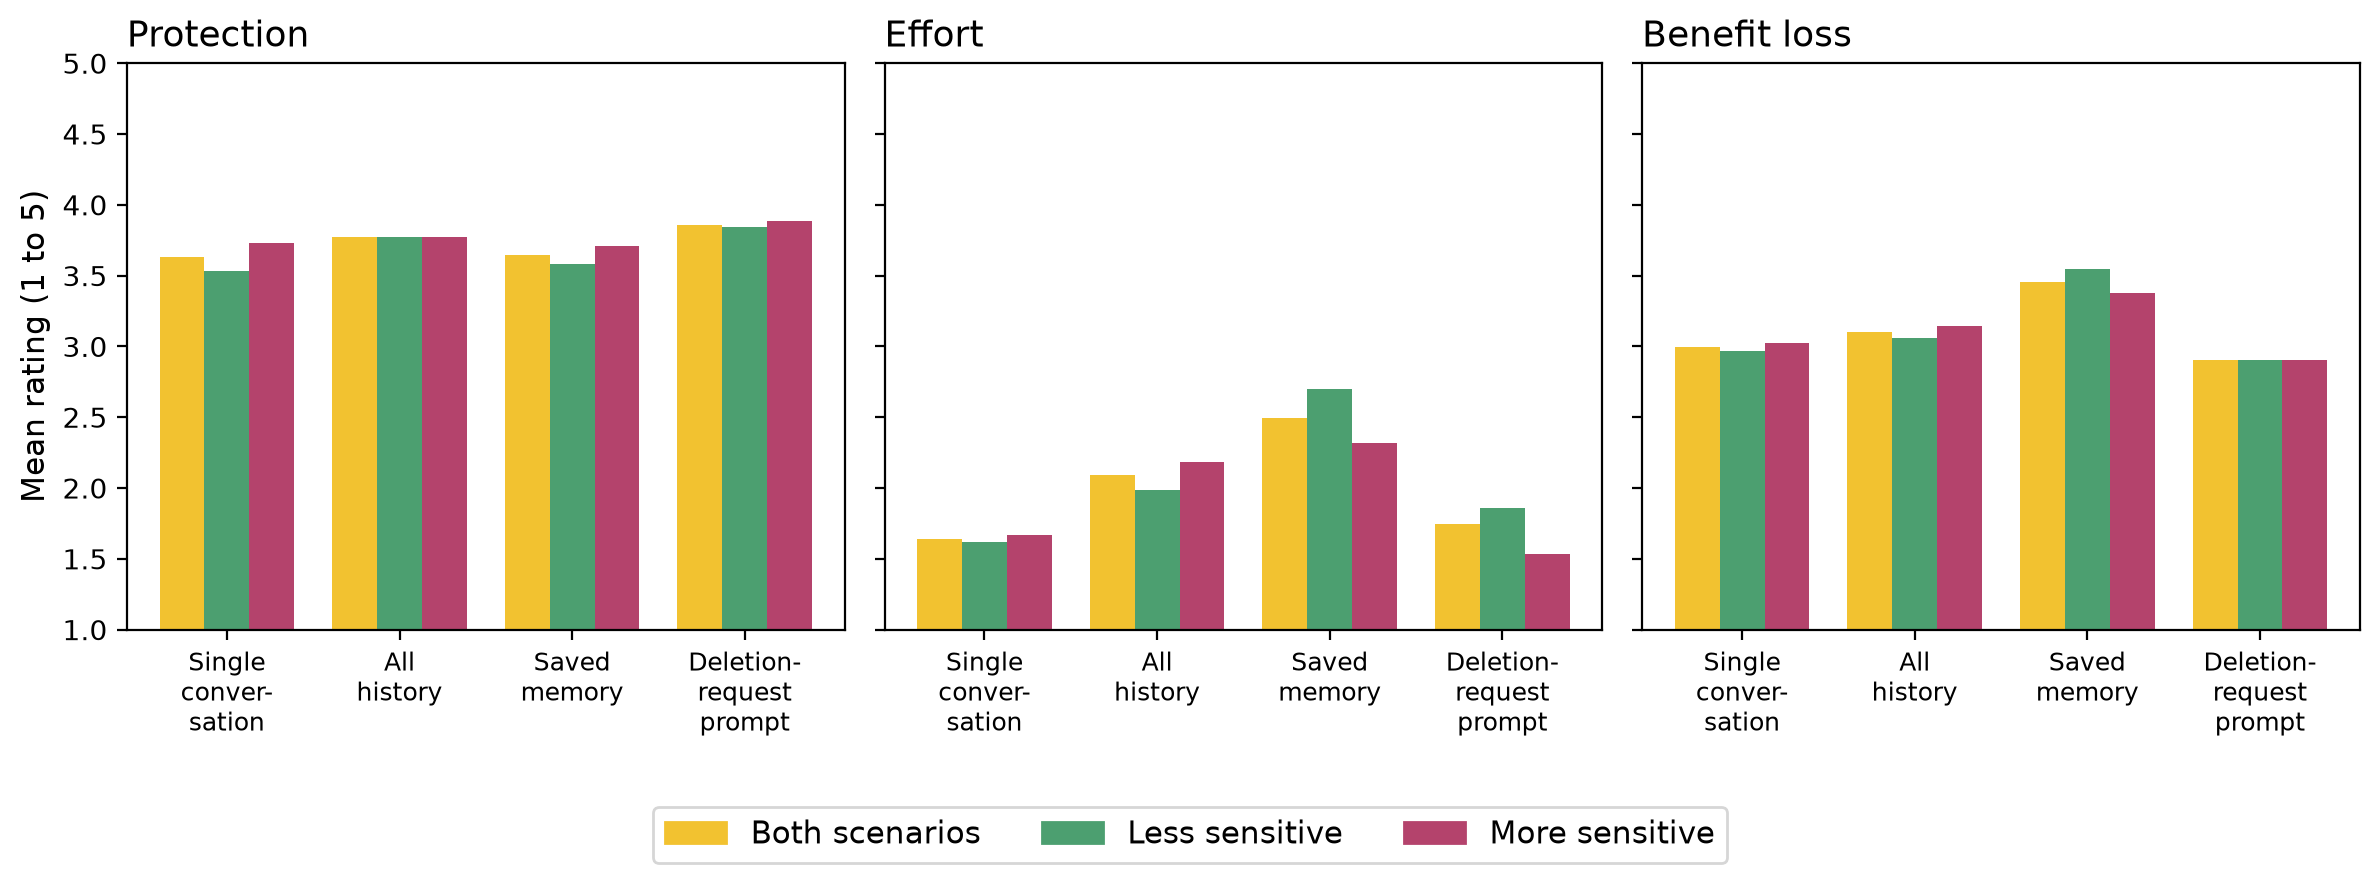
\includegraphics[width=0.9\textwidth]{figures/fig_scales.png}
    \caption{Mean ratings of protection, effort, and benefit loss for the four most chosen methods, for both scenarios combined and for each scenario (317 responses from 105, 50, 30, and 29 participants). Ratings use five-point agreement scales.}
    \label{fig:scales}
\end{figure*}

Many participants could not check that deletion worked, and those who deleted by asking the agent checked by asking the agent. Across Pooled responses, 44.6\% did not know how to check. Those who did check mostly asked the agent, in the same or a new conversation (21\% to 22\% of responses), or looked at the settings or the interface (16\% to 18\%). Participants who deleted by sending a deletion-request prompt checked most often by asking in the same conversation (53.8\% of 39 responses). So for these participants the check is the agent's own answer.

Some participants had seen an agent reference information they believed deleted, and many wanted to know what remained. Of the 177 participants, 42 (23.7\%) had seen this, and 73 (41.2\%) wanted a breakdown of what was deleted and what may be retained. Whether deletion holds up is what the Post-Deletion Behavior section tests (Section~\ref{sec:tech_results}).

\begin{figure}[t]
    \centering
    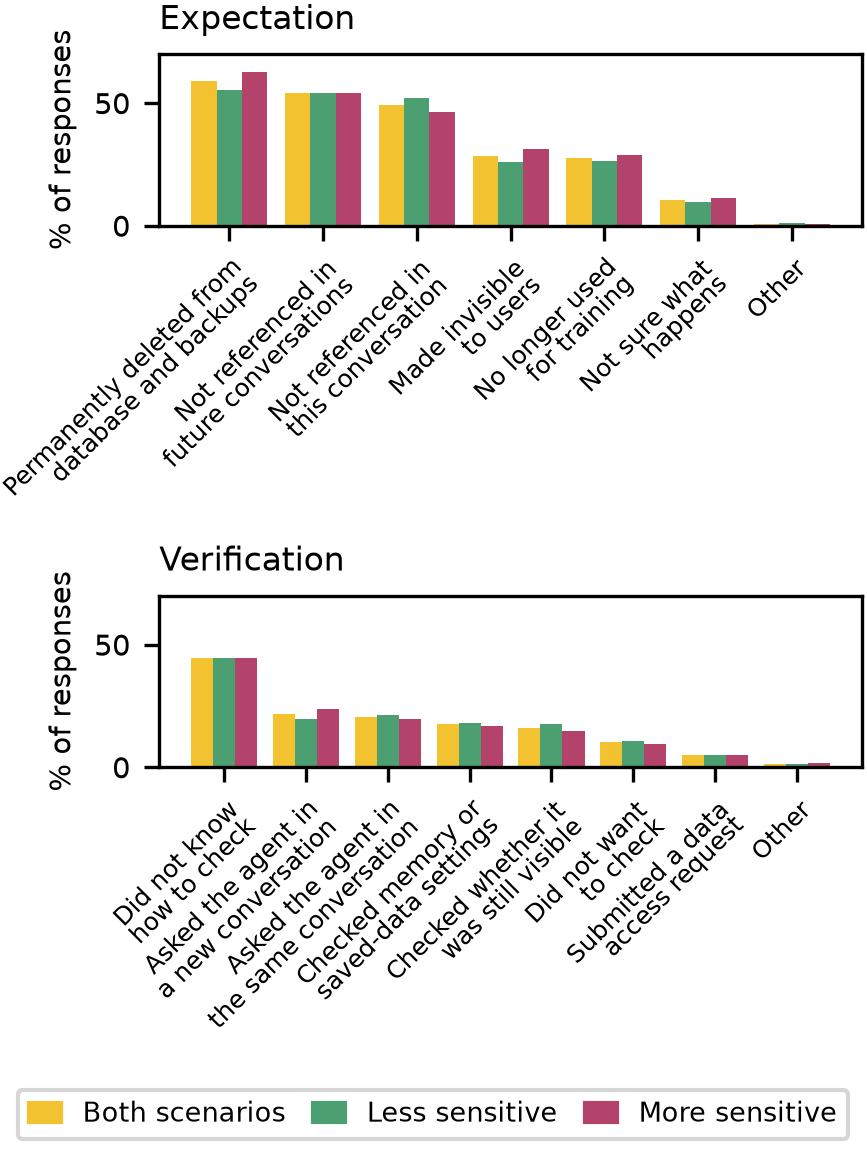
\includegraphics[width=\columnwidth,height=0.42\textheight,keepaspectratio]{figures/fig_expectation.png}
    \caption{Expectations of what deletion does, and how participants checked that it worked, in both scenarios combined and in each scenario (354 responses from 177 participants; participants could select several options). Percentages are of the 354 responses for both scenarios combined and of 177 for each scenario.}
    \label{fig:expectation}
\end{figure}

\FloatBarrier
